\documentclass[11pt,a4paper]{article}
\usepackage[utf8]{inputenc}
\usepackage[spanish]{babel}
\usepackage{amsmath}
\usepackage{amsfonts}
\usepackage{amssymb}
\usepackage{apalike}
\usepackage{graphicx}
\usepackage[left=2cm,right=2cm,top=2cm,bottom=2cm]{geometry}
\title{Circuitos de control de voltaje y corriente con transistores}
\begin{document}

\maketitle


\begin{figure}[h]
\begin{center}

\includegraphics[scale=1]{1.jpeg}
\end{center}
\end{figure}


\begin{center}
\author{Sistemas Electrónicos de Interfaz\\
Barrera Vazquez Omar\\
Ing. Mecatrónica 4B}
\end{center}


\newpage

\section{Objetivo de la practica}

identificar con claridad el uso de transistores en el control de voltaje y corriente el cual esta dado para el control de dispositivos de potencia como lo son los \emph{motores} y otros dispositivos utilizados en la industria.

\section{Materiales a necesitar}

\begin{itemize}

\item 4 MOSFET IRF640N con datasheet
\item 2 Resistencias de 220 $\Omega$
\item 1 Motor inductivo voltaje a consideración de usuario
\item 1 fuente de alimentación con salidas de 5v y 12v
\item 1 circuito de control realizado en la practica 3 (PLC)
\item Cable para unión de \emph{Protoboard}
\item Protoboard donde sera montado el circuito

\end{itemize}


\section{Introducción a controladores de voltaje}
Esta practica esta compuesta por la practica \emph{EV 1-2 optoAcopladores y relevadores}, añadiendo una sección nueva de circuito denomina \textbf{\emph{puente H}}.

\subsection{Puente H}

El puente H es un circuito de control del paso de la corriente, este le da dirección en que circulara la corriente, de modo que los actuadores (motores o luces polarizadas). El puente H trabaja con MOSFET un tipo de transistor que mantiene tres conexiones en su encapsulado, mas adelante hablaremos de eso.

\section{Trabajando con MOSFET}
El trabajar con este tipo de controlador de voltaje y corriente tiene ventajas y desventajas, pero es muy utilizado aun en aplicaciones de potencia por su alta resistencia a temperaturas elevadas así como el trabajar con voltajes elevados.

En esta practica se trabaja con el MOSFET IRF640N con encapsulado To 220AB el cual tiene las siguientes especificaciones tomadas del datasheet del fabricante, como se observa en la figura 1:


\begin{figure}[h]
\begin{center}
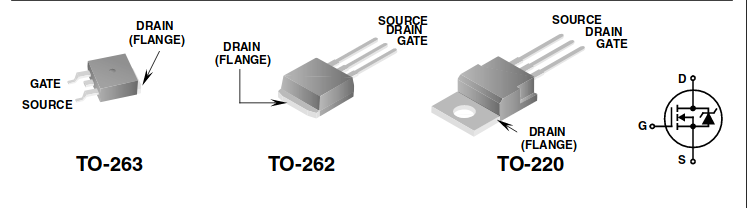
\includegraphics[scale=0.6]{2.png}
\caption{tipos de empaqueta y orden de los pines}
\end{center}
\end{figure}

\newpage

Como se observo en la \emph{figura 1} en mismo tipo de MOSFET maneja tres tipos de encapsulado, por lo que es importante saber que tipo de encapsulado es el que se esta utilizando, mas adelante se observara porque la importancia del empaquetado y conocer su función interna, por lo pronto se observa el orden en que están acomodados los pines. Es básico conocer que un MOSFET tiene tres pines denominados \emph{gate(G), drain(D) y source (S)}, su traducción es español es puerta, drenado y fuente).

Es importante conocer las características con las que trabaja el empaquetado del MOSFET, ya que cada empaquetado puede manejar diferentes tipos de voltajes en cada uno de sus pines, tensiones mas o menos altas así como temperaturas, estos datos técnicos los podemos encontrar en un \emph{datasheet} es una hoja que distribuye el fabricante del componente electrónico el cual nos ayuda a entender sus máximos y mínimos con los que trabaja, así como sus características físicas.

\section{Diagrama de un Puente H}

Como se menciono con anterioridad, el diseño de un \emph{puente H} no es complicado siempre se utilice con claridad los datos técnicos otorgados por el datasheet. A continuación se presenta el diseño de un \emph{puente H} el cual es accionado por dos interruptores y dirección el giro de un motor mediante el control de la circulación de la corriente y voltaje, como se observa el \emph{figura 2}:



\begin{figure}[h]
\begin{center}
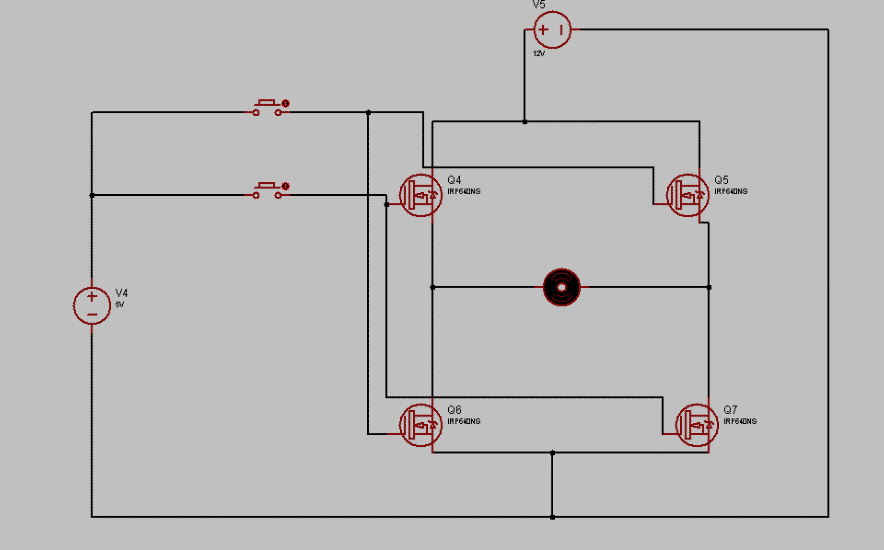
\includegraphics[scale=0.5]{3.png}
\caption{digrama de puente H}
\end{center}
\end{figure}

\subsection{Características del diagrama del puente H}
A pesar de que es un diagrama compuesto por cuatro MOSFET IRF640N los cuales son activados en pares por los \emph{push buttom} y alimentados por una fuente de $V_c$ la cual manda señal a dos MOSFET para dejar fluir la corriente de manera cruzada, esto hará el efecto de dirección, pero mas detalle puedes leer las características que necesita el circuito para funcionar según lo que se este trabajando:

\newpage

\begin{itemize}

\item El diseño del \emph{puente H} funciona con dos fuentes de $I_c$ a 5V para pulso eléctrico del \emph{GATE} y una mas que sera la que alimente el motor, esta dependerá el voltaje que el motor maneje, checarlo en la hoja de datos correspondiente al motor.

\item Dos de los MOSFET son activados en manera par y cruzada por un push button, esto para que el cambio de giro sea correcto de lo contrario el motor ni siquiera funcionara

\item El \emph{voltaje positivo} entra por el Source y sale por pin denominado Drain, después se dirección a una entrada del motor

\item En la simulación con \emph{software} al ponerlo en funcionamiento hace el cambio de giro inmediatamente, pero al armar el circuito tiene un problema, tarda en detener el giro y hacer el cambio de tal, por lo que se agrega una \emph{resistencia de descarga} esto se observara en la siguiente apartado.

\end{itemize}

\section{Circuito de puente H}
En el circuito armado de la figura 3, podemos observar el armado del diagrama de la figura 2, en el cual se observa una agregación de una resistencia que conecta el nodo de la entrada del \emph{gate} y el positivo de la fuente, direccionando hacia el negativo de la fuente que alimenta el circuito, esto permitirá que se descargue de manera inmediata la alimentación, por lo que no tardara en detener el giro.\cite{munoz2016ensenando}


\begin{figure}[h]
\begin{center}
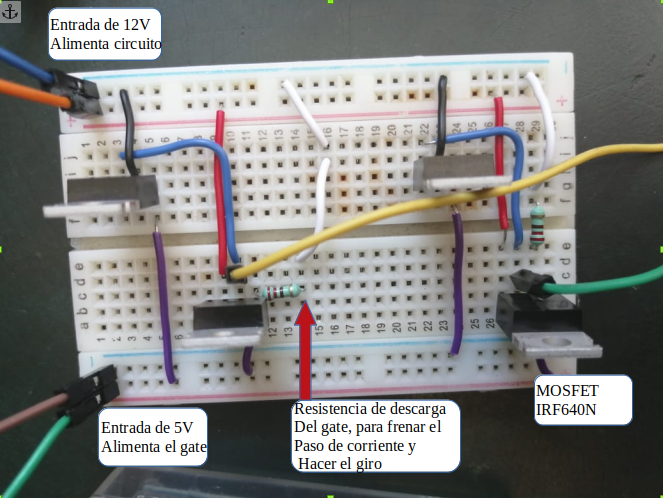
\includegraphics[scale=0.4]{4.png}
\caption{circuito armado puente H}
\end{center}
\end{figure}

La practica concluye con las siguientes determinaciones:
\begin{itemize}
\item es necesario conocer los datos técnicos de los componentes
\item saber solucionar cuestiones de corriente en un puente H
\item determinar voltajes y corrientes dentro del circuito
\item hacer las conexiones lo mas limpio posible para evitar problemas de cortos u otros
\end{itemize}


\bibliographystyle{apalike} 
\bibliography{ref}






\end{document}